%!TEX root=../document.tex

\section{Begriffe und Definition - Einführung}

	\subsection{Was versteht man unter Qualität? Geben Sie einen der beiden gehörten/gelernten Definitionen}
	
		Qualität ist die vollständige Erfüllung aller vertraglich vereinbarten Eigenschaften eines Produktes und oder einer Dienstleistung für einen definierten festgelegten Verwendungszweck.
	

	\subsection{Ist Qualität quantifizierbar - etwa auf einer Werteskala von 1-10?}

	\subsection{Ist ausreichende Qualität bezüglich eines Produktes/einer Dienstleistung für einen Kunden übertragbar auf alle anderen?}
	

	\subsection{Was versteht man unter Management?}
	
		Unter Management versteht man das Planen, Verwalten, sowie das kontrollierte Einsetzen von Ressourcen (HR, Geld, Rohstoffe, Zeit, ...)

	\subsection{Was versteht man unter Qualitätsmanagement - und welche Tätigkeiten gehören dazu?}
	QM ist die Summe aller Tätigkeiten die zur Einhaltung/Erzeugung einer Dienstleistung oder Ware beitragen.
	Aufgaben im Qualitätsmanagement:
	\begin{itemize}
		\item Qualitätsplanung:
			\subitem dient zur Erfüllung aller zuvor festgelegten Ziele, dabei sind die erforderlichen Prozesse, verfügbaren finanziellen Mittel immer zu berücksichtigen.
		\item Qualitätslenkung:
			\subitem trägt zur Beseitigung von Fehlerursachen bei und Überwacht den Produktionsablauf.
		\item Qualitätssicherung:
			\subitem überwacht und bestätigt die Angeforderten Qualitätsanforderungen im gesamten Fertigungsprozess um den Standard des Produkts zu erfüllen.
		\item Qualitätsverbesserung:
			\subitem beschäftigt sich mit allen Aufgaben die den Kunden zufriedenstellen und dienen der kontinuierlichen Verbesserung.
	\end{itemize}

	\subsection{Nennen Sie die beiden übergeordneten strategischen Ziele jedes normgerechten Qualitätsmanagementsystems.}
	
	\begin{itemize}
		\item Verlässliche Qualtität einer Dienstleistung,
		\item Nachweis über verlässliche Qualität,
		\item Weiterentwicklung der Qualität,
	\end{itemize}
	
	Übereinstimmung von Produkteigenschaften mit den Anforderungen und den Erwartungen der KundInnen
	
	Maß der	Übereinstimmung von Leistungsversprechen und Leistungserbringung	

	\subsection{Skizzieren Sie den Werdegang (inklusive Abhängigkeiten) eines Produktes bzw. einer Dienstleistung von der Planung über die Produktion bis zum Kunden ( Skizze mit erläuternden Stichworten) }

	\subsection{Reicht die strenge Selektion von Einheiten innerhalb des Toleranzbereiches nach der Produktion als ausreichende Maßnahme im Qualitätsmanagement? Wenn nein, warum nicht?}

	\subsection{Was hat Qualitätsmanagement mit Regelkreisen zu tun? welche systemimmanenten Regelkreise muss ein funktionierendes Qualitätsmanagementsystem haben?}
	
	\begin{itemize}
		\item \textbf{Steuern}: ohne Rückmeldung (normal bremsen),
		\item \textbf{Regeln}: Mit (sensorischer) Rückmeldung (ABS),
		\item \textbf{Organisation}: beinhaltet die Prozesskette und bringt das Produkt zum Kunden,
		\item \textbf{Prozesskette}: Input -> PROZESS -> Output ist INPUT -> PROZESS -> Output ..,
	\end{itemize}
	
	\begin{itemize}
		\item Kleiner Regelkreis zwischen PR/DL und Prozesskette.
		\item Kleiner Regelkreis zwischen Prozesskette und Organisation.
		\item Großer Regelkreis zwischen  Organisation und Kunden.
	\end{itemize}
	
	\begin{itemize}
		\item Ausstoß: Menge die man produziert.
		\item Ausschuss: Menge die defekt ist.
	\end{itemize}

	\subsection{An welchen Stellen eines Prozesses bzw. einer Prozesskette können bzw. müssen sie Überprüfungen der Qualität durchführen?}

	\subsection{Geben Sie das international übliche „Blockschaltbild“ eines Regelkreises mit allen Standardbezeichnungen an.}
	
	\begin{itemize}
		\item 1.Regler
		\item 2.Stelleinrichtung
		\item 3.Regelstrecke
		\item 4.Messeinrichtung
	\end{itemize}
	\begin{figure}[!h]
		\begin{center}
			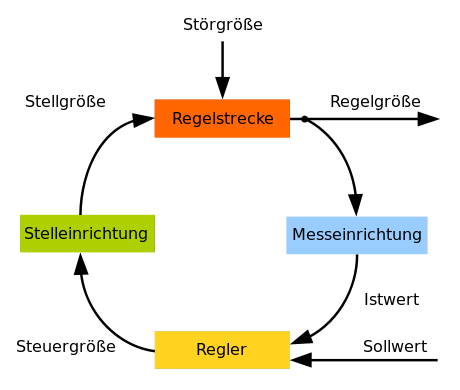
\includegraphics[width=0.68\linewidth]{images/blockschaltbild}
			\caption{Blockschaltbild Regelkreistechnik}
		\end{center}
	\end{figure}

	\subsection{Wodurch unterscheiden sich Steuerung und Regelung?}

	\textbf{Unterschied zwischen Steuerung und Regelung nach DIN 19226 }
	
	Eine Regelung ist ein Zusammenspiel aus stetiger Messung und der Steuerung eines Systems in Abhängigkeit einer Vorgabe. \newline
	Im Unterschied zur Regelung fehlt bei einer Steuerung die Rückwirkung der Ausgangs-Größen auf die Eingangs-Größen. \newline
	Bei der Regelung gibt es eine Rückwirkung, indem ein ständiger Vergleich von Soll und Ist stattfindet. Die Wirkungsweise kann man sich anhand einer Heizung vorstellen: Man möchte eine konstante Zimmer-Temperatur von 20 Grad erhalten. Per Thermostat wird ständig die Temperatur gemessen und bei Unterschreiten und Überschreiten meiner vorgegebenen 20 Grad die Warmwasserzufuhr entsprechend geregelt. 
	
	\subsection{Was versteht man im Qualitätsmanagement unter einem Prozessmodell - geben Sie ein Beispiel mittels einer kurzen Prozesskette an.}

		\begin{figure}[!h]
			\begin{center}
				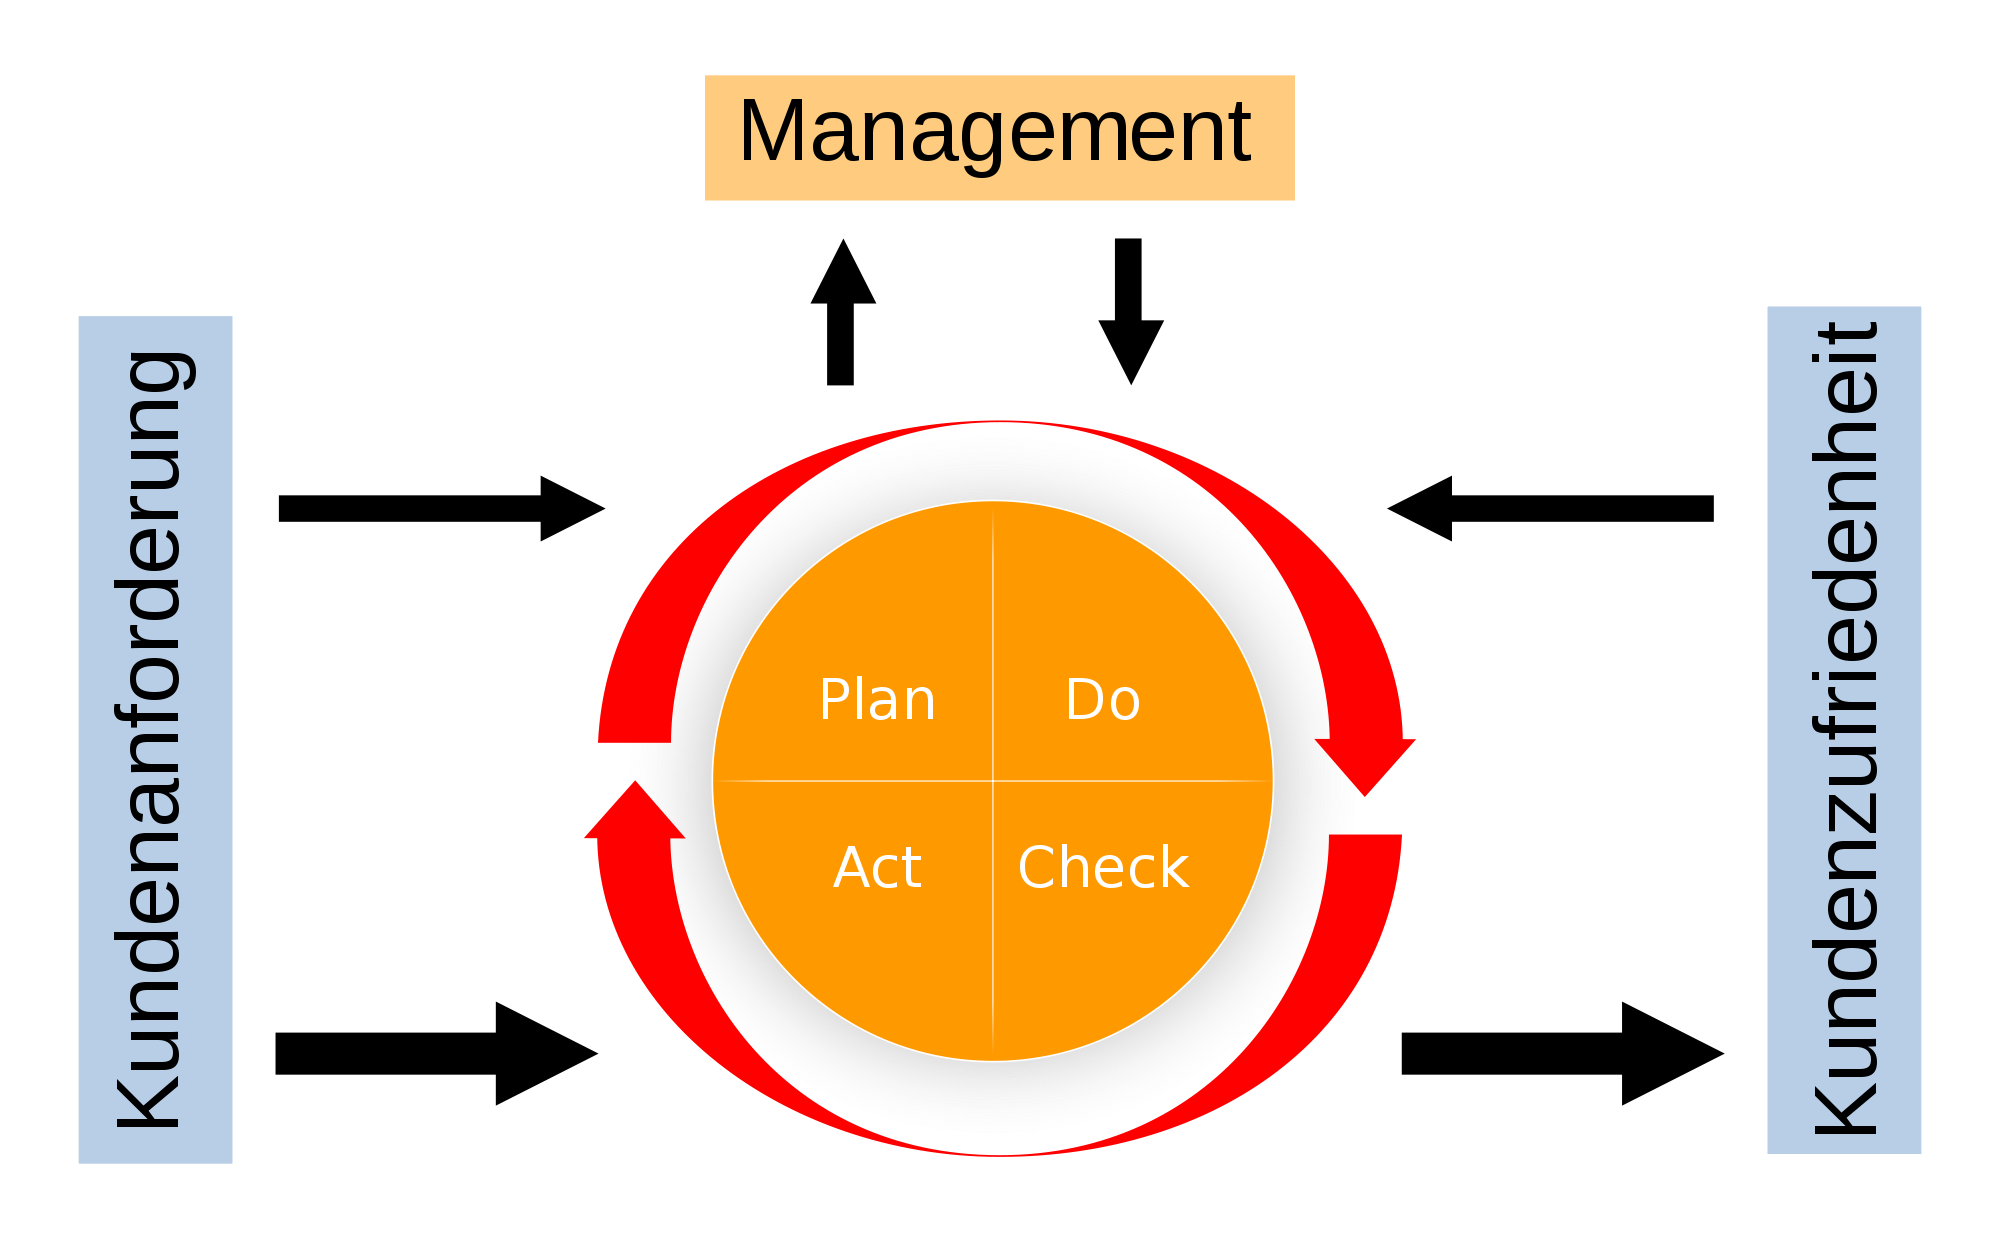
\includegraphics[width=0.68\linewidth]{images/prozessmodel}
				\caption{kleine Prozesskette}
			\end{center}
		\end{figure}
	\subsection{Skizzieren Sie die Prozesskette von der Schnittstelle mit ihrem Lieferanten bis zur Schnittstelle mit ihren Kunden und geben Sie an, welche (Mindest-)Prüfungen verpflichtend sind und welche Verpflichtung für ihre Lieferanten und sie (als zertifizierte Organisation) sich daraus ableiten.}

\section{Motivationsgründe und Einführung eines normkonformen Qualitätsmanagementsystems}

	\subsection{Nennen Sie alle Motivationsgründe, warum eine Firma bzw. Organisation ein standardisiertes Qualitätsmanagementsystem einführen und erhalten sollte.}
	
	\begin{itemize}
		\item Wettbewerbsfähigkeit, durch Ausgangsprüfung
		\item glaubwürdige Lieferanten, durch Stichproben
		\item Abwehr von ungerechtfertigten Schadenersatzansprüchen, durch Rückführbarkeit
		\item Zertifikat lässt Erwartungen steigen
		\item gesetzliche Auflagen (CE-Prüfzeichen)
	\end{itemize}
	
	\subsection{Stellen Sie die Vorgehensweise bei Umsetzung eines normkonformen Qualitätsmanagementsystems in einem bestehenden Betrieb bis zur Zertifizierung bzw. Rezertifizierung dar.}
	
	\subsection{Auf welcher Tatsache beruht - bei richtiger Umsetzung - die Analogie: Qualitätsmanagement = ordentliches Betriebsmanagement? }
	
	\subsection{Gibt es Gründe, weshalb der Gesetzgeber die Einrichtung und Erhaltung eines vollständigen und zertifizierten Qualitätsmanagementsystems zwingend einfordern kann - mit welchen Konsequenzen? }
	
	\subsection{Was versteht man unter CE - Ist CE ein Qualitätszeichen?}
	
	\subsection{Nennen Sie die beiden übergeordneten strategischen Ziele jedes normgerechten Qualitätsmanagementsystems.}
	
	\subsection{Auf welcher Tatsache beruht - bei richtiger Umsetzung - die Analogie: Qualitätsmanagement = ordentliches Betriebsmanagement? }
	
	\subsection{Woraus und wie werden die Vorgaben von Qualitätszielen abgeleitet und wodurch wird der Grad der Zielerreichung nach Ablauf der Beobachtungsperiode nachweisbar. – Nennen Sie EIN Beispiel.}
	
\section{Normkonformes Dokumentensystem}
	
	\subsection{Aus welchen Arten von Dokumenten besteht ein QM-Dokumentensystem und welche Funktionen haben die Dokumente? – Gemeinsamkeiten und Abgrenzungen?}
	
	\subsection{Was versteht man unter einem QM-Handbuch und wozu wird es verwendet?}
	
	\subsection{Welche formalen Merkmale muss eine aktuell gültige Verfahrensanweisung besitzen, um normgerecht zu sein (QMA bzw QMV) – Dokumentenstatus}
	
	\subsection{Wie sieht die Struktur einer QMV = Verfahrensanweisung aus und welchenAusgabenstatus kann das Dokument haben?}
	
	\subsection{Welche Merkmale muss eine normgerechte Arbeitsanweisung aufweisen? A: Dokustatus mit Titel , Ordnungsbegriff, Versionsnummer, Freigaberahmen, Seitennummer, ….  sowie den 9 Punkten: Zweck, Gültigkeitsbereich= EIN ARBEITSPLATZ, Definitionen, ……}
	
	\subsection{Wie wird eine Änderung in einem QM-Dokument  richtig umgesetzt?
	A. neue Version mit allen Seiten neu in Umlauf gesetzt– kein Austausch einzelner Seiten! alte Version zurückgezogen = Original auf erster Seite einfach durchgestrichen und mit Text: am <Datum> zurückgezogen/ersetzt durch v2; Einsammeln der alten Versions-Kopien und Vernichtung}

